\begin{figure}[H]
\centering
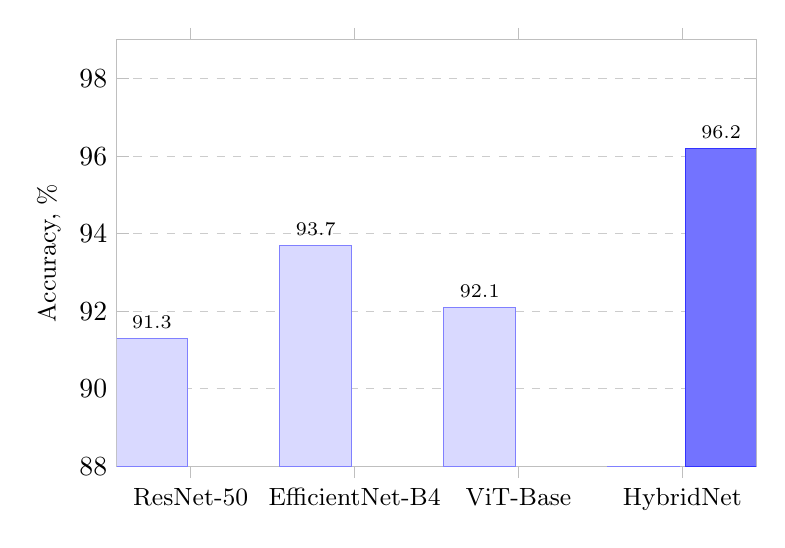
\begin{tikzpicture}
\begin{axis}[
  ybar,
  width       = 0.80\textwidth,
  height      = 7cm,
  bar width   = 26pt,
  symbolic x coords = {ResNet-50, EfficientNet-B4, ViT-Base, HybridNet},
  xtick       = data,
  xticklabel style = {font=\small},
  ymin = 88, ymax = 99,
  ylabel      = {Accuracy, \%},
  ylabel style= {font=\small},
  ytick       = {88,90,92,94,96,98},
  ymajorgrids = true,
  grid style  = {dashed, gray!40},
  nodes near coords,
  nodes near coords style = {font=\scriptsize\bfseries, anchor=south},
  axis line style = {gray!50},
  tick style      = {gray!50},
  enlarge x limits = 0.15,
]
  \addplot[fill=blue!15, draw=blue!50]
    coordinates {
      (ResNet-50,91.3)(EfficientNet-B4,93.7)(ViT-Base,92.1)(HybridNet,0)
    };
  \addplot[fill=blue!55, draw=blue!80]
    coordinates { (HybridNet,96.2) };
\end{axis}
\end{tikzpicture}
\caption{Порівняння методів за метрикою Accuracy на датасеті ChestX-ray14}
\label{fig:chart}
\end{figure}
